\documentclass[a4paper, oneside, 12pt]{article}

%%%%%%%%%% Paquets %%%%%%%%%%

% Paquets pour le Français
\usepackage[utf8]{inputenc} % Gestion encodages
\usepackage[T1]{fontenc} % ???
\usepackage[francais]{babel} % Typographie française

\usepackage{cleveref}

% Images
\usepackage{graphicx}

% Mise en page
\usepackage[top=2.5cm, bottom=7.5cm, left=2.5cm, right=2.5cm, footskip=4.5cm]{geometry}

% Outils pour l’écriture
\usepackage{xcolor} % Utilisé pour les hiddeux \todo
\usepackage{layout} % Pour voir les commandes utiles

% Couleurs
\usepackage{color}
\definecolor{coloration_numero_ligne}{gray}{0.6}
\definecolor{coloration_reglette}{gray}{0.5}
\definecolor{coloration_fond}{rgb}{1, 1, 1}
\definecolor{coloration_commentaire}{rgb}{0, 0, 0.9}
\definecolor{coloration_mot_cle}{rgb}{0.75, 0, 0}
\definecolor{coloration_chaine}{rgb}{1, 0.2, 1}
\definecolor{coloration_type}{rgb}{0, 0.7, 0}
\definecolor{coloration_erreurs}{rgb}{0.6, 0.35, 0.8}

% Tabulations verbatim
% http://www.grappa.univ-lille3.fr/FAQ-LaTeX/6.16.html
\makeatletter
{\catcode`\^^I=\active
\gdef\verbatim{\catcode`\^^I=\active\def^^I{\hspace*{4em}}%
\@verbatim \frenchspacing\@vobeyspaces \@xverbatim}}
\makeatother

% Coloration syntaxique
\usepackage{minted}
\newminted[shellcode]{shell}{tabsize=4,xleftmargin=1cm,fontsize=\footnotesize,frame=leftline}
% On trouvera probablement difficilement mieux…
\newminted[kamcf]{ini}{tabsize=4,xleftmargin=1cm,fontsize=\footnotesize,frame=leftline}

%%%%%%%%%% Commandes supplémentaires %%%%%%%%%%%

% Marquage du travail restant
% [#1] Texte à afficher
\newcommand{\todo}[1][Il y a là encore des choses à écrire !]{\colorbox{yellow}{#1}}

%%% Gestion du sommaire
% Section non numérotée
% {#1} Nom de la section
\newcommand{\sectionSpeciale}[1]{\section*{#1}\addcontentsline{toc}{section}{#1}}
% Section non numérotée dont le titre n’est pas affiché.
% {#1} Nom de la section
\newcommand{\sectionCachee}[1]{\addcontentsline{toc}{section}{#1}}

%%% Gestion des annexes
\makeatletter
	
	\newcounter{annctr}
	
	% Définir une annexe
	% {#1} Nom de l’annexe
	\newcommand{\annexe}[1]{\stepcounter{annctr}\addcontentsline{ann}{section}{\protect\numberline {\Alph{annctr}}#1}\section*{\numberline {\Alph{annctr}}#1}}
	% Lister les annexes
	% Note : ce serait quand même bien de le faire fonctionner sans avoir besoin du makefile.
	\newcommand\listeannexes{\sectionSpeciale{Annexes}\input{annexes.tex}}
	
	% Déclaration et ouverture du fichier de stockage de la liste des annexes
	\newwrite\tf@ann
	\immediate\openout\tf@ann\jobname.ann\relax
      
\makeatother

%%%%%%%%%% Abréviations %%%%%%%%%%
% Le contenu suffit comme documentation…

\newcommand\win{Windows}
\newcommand\mac{Mac}
\newcommand\lnx{Linux}
\newcommand\lnp{Linphone}

\newcommand\my{MySQL}
\newcommand\kam{Kamailio}
\newcommand\rad{RADIUS}
\newcommand\frad{FreeRADIUS}
\newcommand\apa{Apache}
\newcommand\pma{phpMyAdmin}
\newcommand\xlite{X-Lite}
\newcommand\cph{Cisco phone \todo[(remplacer par la référence)]}
\newcommand\ata{ATA}


\begin{document}

%%% Page de garde %%%

% Pas de numéro sur cette page
\thispagestyle{empty}

% Note : logo disponibles sur http://fc.isima.fr/~brunot/files/isima/logos/
% J’avais trouvé une version vectorielle, ce serait mieux, mais je ne la trouve plus…

\includegraphics[width=6cm]{isima.png}

\vspace{0.5cm}

\begin{minipage}{4cm}
\begin{flushleft}
	Institut Supérieur d’informatique, de Modélisation et de leurs Applications
	
	\vspace{0.5cm}
	
	\small{ Campus des Cézeaux \\ 24 rue des Landais \\ BP 10125 \\ 63173 Aubière CEDEX }
\end{flushleft}
\end{minipage}

\vspace{4cm}

\begin{center}
	Rapport d’ingénieur \\
	Projet de 2{\ieme} année \\
	Filière {\em{Réseaux et télécommunications}} \\
	\Large{Facturation d’appels sur un serveur Kamailio/Radius}
\end{center}

\vspace{2cm}

\large{
\begin{tabular}{ll}
\textit{Présenté par :} & \textbf{Lucien Guimier} \\
& \textbf{Damien Teyssier}
\end{tabular}
}

\todo

\newpage
	
%%% Avant-propos %%%
\pagenumbering{roman}

\sectionSpeciale{Remerciements}

\todo
\newpage

\renewcommand{\listfigurename}{Table des illustrations}
\renewcommand{\figurename}{{\sc Illustration}}
\sectionCachee{\listfigurename}
\listoffigures
\newpage

\sectionSpeciale{Résumé}

\todo

\vspace{10cm}

\sectionSpeciale{Abstract}

\todo
\newpage

\renewcommand{\contentsname}{Table des matières}
\sectionCachee{\contentsname}
\tableofcontents
\newpage

% Sauvegarde du numéro de la page courante
\newcounter{metapage}
\setcounter{metapage}{\value{page}}
% Remise à zéro des numéros de page & changement de chiffres
\pagenumbering{arabic}

%%% Contenu %%%

\sectionSpeciale{Introduction}

La VoIP est devenue l'avenir de nos conversations téléphoniques. En effet, la téléphonie commutée (dite classique) est vouée à disparaitre dans un avenir proche. Dans le milieu des entreprises, la VoIP est aujourd'hui majoritaire même si la transition fût difficile à cause des coûts qu'elle demandait aux entreprises. Cependant, cette solution a un avantage de coût à long terme puisque qu'elle permet de faire passer toutes les communications sur le réseau de transfert de données et ainsi réduire les coûts de communication.

C'est pour cette raison que l'on nous a demandé de continuer le projet de madame Salimata \nom{Ndiaye} et monsieur Quentin \nom{Volant}. On a donc dû suivre leur protocole afin de pouvoir remonter un serveur de téléphonie en VoIP {\kam} et un serveur d'authentification {\rad}.

Nous devions ainsi réécrire une procédure d'installation de ces serveurs et, ensuite, coder une application de facturation des communications VoIP pouvant être utilisée par une entreprise.

Dans un premier temps, nous allons voir notre protocole d'installation des serveurs {\kam} et {\frad}. Nous allons ensuite expliquer les différents outils de communication que nous avons essayés d'utilisés sur notre serveur. Finalement, nous présenterons le fonctionnement de l'application de facturation.
\newpage

% Première section : installation de serveurs
\section{Installation}

\subsection{Installation du système}

\todo[Trouver la version de Debian]

La première étape de notre projet consistait en l’installation de serveurs de téléphonie SIP. Nous en avons installé deux, fontionnant avec le système d’exploitation Debian. Conformément à notre cahier des charges, nous y avons installé un proxy SIP, {\kam}, attaché à un serveur d’authentification {\rad}, {\frad}.

\subsection{\kam}

\subsubsection{Installation}

Pour installer {\kam}, il nous a fallu commencer par installer les dépendances qui n’étaient pas encore présentes dans le système, disponibles dans les paquets :

\begin{itemize}
	\item{gcc} ;
	\item{bison} ;
	\item{libmysqlclient-dev} ;
	\item{libradiusclient-ng-dev} ;
	\item{mysql-server} ;
	\item{mysql-client} ;
	\item{make}.
\end{itemize}

Nous avions initialement envisagé d’utiliser ensuite les paquets Debian disponibles sur les serveurs de {\kam}, mais le paquet de base n’est pas compilé avec le support de {\rad}, rendant le paquet des bibliothèques d’authentification {\rad} inopérant.

Nous avons donc téléchargé et décompressé les sources de {\kam} pour les compiler. Nous avons choisi d’utiliser la dernière version disponible, qui était la version 4.2.2. Pour cela, nous avons utilisé les commandes :

\begin{shellcode}
wget http://www.kamailio.org/pub/kamailio/4.2.2/src/kamailio-4.2.2_src.tar.gz
tar xvf kamailio-4.2.2_src.tar.gz
\end{shellcode}

Puis nous sommes allés dans le dossier ainsi créé, pour notre part kamailio-4.2.2 et nous avons exécuté :

\begin{shellcode}
make cfg
\end{shellcode}

Cette commande construit la configuration par défaut pour la compilation, qu’il a fallu adapter à nos besoins. Conformément aux indications du rapport de l’année dernière, nous avons effectué les modifications suivantes :

\begin{itemize}
	\item{dans la liste de modules exclus du fichier \texttt{module.lst}, nous avons retiré les noms des modules concernant {\my} et {\rad}}.
\end{itemize}

Nuos avons ensuite compilé et installé {\kam} :
	
\begin{shellcode}
make all
make install
\end{shellcode}

Cette dernière commande installe {\kam} dans \texttt{/usr/local}.

\subsubsection{Configuration}

Nous avons dû ensuite configurer {\kam}. Nous sommes allés dans le dossier \texttt{/usr/local/etc/kamailio}. Il a fallu rajouter les lignes suivantes dans le fichier de configuration \texttt{kamailio.cfg} :

\#!define WITH\_MYSQL

\#!define WITH\_AUTH

\#!define WITH\_USRLOCDB

\#!define WITH\_NAT

Nous avons alors créé puis configuré la base de données. Pour la créer, il a fallu d'abord préciser quel système de base de données nous allions utiliser.
Dans notre cas, c'est mysql. C'est pourquoi il a fallu aller dans le fichier \texttt{/usr/local/etc/kamailio/kamctlrc} afin de décommenter la ligne :

DBENGINE=MYSQL

Ensuite, nous avons tapé 
\begin{shellcode}
/usr/local/sbin/kamdbctl create
\end{shellcode}
\todo

\subsection{\frad}
\subsubsection{Installation}

Nous avons choisi ensuite d'installer {\frad} à partir des paquets présents sur la machine. Pour cela, il a fallu taper la commande :

\begin{shellcode}
apt-get install freeradius
\end{shellcode}

Il fallait aussi installer les outils nécessaires au bon fonctionnement de {\frad} :

\begin{shellcode}
apt-get install freeradius-utils
\end{shellcode}

Puis, pour finir, nous avons installé un client Radius nommé Radiusclient grâce à la commande suivante :

\begin{shellcode}
apt-get install radiusclient1
\end{shellcode}

\subsubsection{Configuration}
Nous avions fini d'installer {\frad}. Il nous restait donc à le configurer. Ce serveur {\rad} peut être configuré de deux manières différentes. Soit à partir des fichiers présents dans \texttt{/etc/freeradius}, soit à partir d'une base de données. Nous avons choisi de configurer à partir des fichiers. Il a donc fallu aller vérifier si la configuration se faisait bien grâce aux fichiers. Pour cela, il a suffi d'aller vérifier dans le fichier \texttt{/etc/freeradius/sites-available/default}.

Ensuite, nous sommes allés dans le répertoire \texttt{/etc/freeradius} afin de modifier le fichier \texttt{users}. Dans ce fichier, nous avons ajouté des utilisateurs de la façon suivantes :

login Cleartext-Password:="password"

Cette ligne autorise l'utilisateur login à se connecter avec le mot de passe "password".

Nous avons pû ensuite faire le test en utilisant la commande suivante :

\begin{shellcode}
radtest login password localhost 0 testing123
\end{shellcode}

Le paramètre "testing123" est le mot de passe donné par défaut au client localhost dans le fichier \texttt{/etc/freeradius/client.conf}. Nous l'avons ensuite changé en "kamailio".


\subsubsection{Intégration de {\rad} à {\kam}}

Pour commencer, il a fallu copier les dictionnaires \texttt{/usr/local/etc/kamailio/dictionary.kamailio} et \texttt{/usr/local/etc/kamailio/dictionary.sip} dans le répertoire \texttt{/etc/radiusclient-ng}.

\begin{shellcode}
cp /usr/local/etc/kamailio/dictionary.kamailio /etc/radiusclient-ng

cp /usr/local/etc/kamailio/dictionary.sip /etc/radiusclient-ng
\end{shellcode}

Puis, nous avons inclus dans \texttt{/etc/radiusclient-ng/dictionary} les deux fichiers suivants :

\begin{itemize}
\item{\texttt{/etc/radiusclient-ng/dictionary.kamailio}}
\item{\texttt{/etc/radiusclient-ng/dictionary.sip}}
\end{itemize}

Puis il a fallu décommenter les lignes des attributs ou des valeurs Failed, Sip-Session et Call-Check dans les trois fichiers dictionary.

Nous avons ensuite dû vérifier que les deux lignes suivantes,qui donnent l'adresse du serveur {\rad}, se trouvaient bien dans le fichier \texttt{/etc/radiusclient-ng/radiusclient.conf} :

\begin{itemize}
\item{authserver localhost}
\item{acctserver localhost}
\end{itemize}

Nous avons ensuite été modifier le fichier \texttt{/etc/radiusclient-ng/servers}. Nous avons annoncé notre serveur de la façon suivante :


192.168.102.120		kamailio


Ce fichier contient l'adresse des serveurs {\rad} et leurs clefs. Ainsi nous avons choisi la clef "kamailio".

Puis ensuite il a fallu aller modifier le fichier \texttt{/etc/freeradius/clients.conf} qui définit les clients autorisés par le serveur {\frad} :

\begin{shellcode}
Client localhost
{
 ipaddress = 192.168.102.120
 secret = kamailio
}
\end{shellcode}

Nous avons dû ensuite modifier le fichier \texttt{/etc/freeradius/users}. Nous avons tout effacer et avons écrit les utilisateurs autorisés ou pas de la manière suivante :


7000@192.168.102.120 Auth-Type=Accept
7001@192.168.102.120 Auth-Type=Accept
7003@192.168.102.120 Auth-Type=Reject


Cela autorise les utilisateurs 7000 et 7001 mais rejette l'utilisateur 7002.

Ainsi nous avons deux sécurités à passer afin de pouvoir utiliser le serveur {\kam}. Il faut tout d'abord être dans la base de donnée de {\kam} puis ensuite dans le fichier users de {\frad} en tant qu'utilisateur accepté.



\newpage

\sectionSpeciale{Conclusion}

Il nous été demandé d'installer une solution de téléphonie SIP utilisant un proxy SIP {\kam} ainsi qu'un serveur d'authentification {\rad} {\frad}. Nous devions ensuite créer une application de facturation en utilisant les journaux de {\frad}. Durant toute la durée de notre projet, nous avons pu utiliser le matériel fourni par l'ISIMA.

Les principaux problèmes que nous avons rencontrés durant la durée de notre projet sont lié à la recherche de documentation. En effet, nous avons perdu beaucoup de temps sur ces recherches. 

Finalement, nous sommes parvenus à installer deux serveurs entre lesquels nous avons pu communiquer. Suite au montage du second serveur, nous avons réécrit une nouvelle procédure d'installation des serveurs.  
Nous avons également codé et utilisé l'application de facturation demandée.
Nous aurions cependant aimé pouvoir mieux résoudre le problème de droits des journaux d'appels de {\frad} et mieux gérer la nécessité d'utiliser des adresses IP pour l'{\ata}.


\newpage

%%% Après-propos %%%

% Changement des chiffres utilisés pour les numéros de pages
\pagenumbering{roman}
% Rétablissement du numéro de page méta
\setcounter{page}{\value{metapage}}

\sectionSpeciale{Références}

\subsection*{Référence bibliographique}

\noindent[1] Salimata \nom{Ndiaye} et Quentin \nom{Volant}, \textit{Rapport de projet de 2\up{nde} année}, ISIMA, Aubière, 2014.

\subsection*{Webographie}

\noindent[2] \textit{Kamailio SIP Server v4.2.x (stable): Pseudo-Variables}, disponible sur : \url{http://www.kamailio.org/wiki/cookbooks/4.2.x/pseudovariables}

\noindent[3] \textit{ACC\_RADIUS Module}, disponible sur : \url{http://www.kamailio.org/docs/modules/4.2.x/modules/acc_radius.html}

\newpage

% Annexes
\listeannexes

\annexe{Diagramme de classes de la manipulation du journal}
\begin{center}
	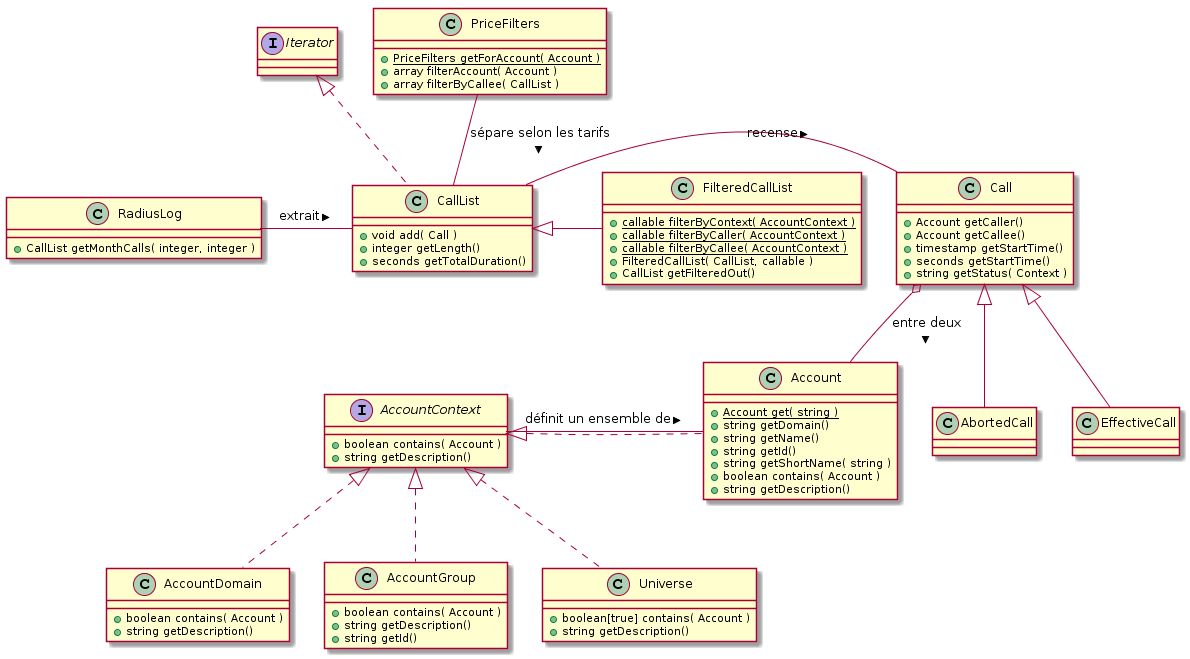
\includegraphics[angle=90, height=18cm]{uml/calls.png}
\end{center}

\annexe{Diagramme de classes de la construction de pages}
\begin{center}
	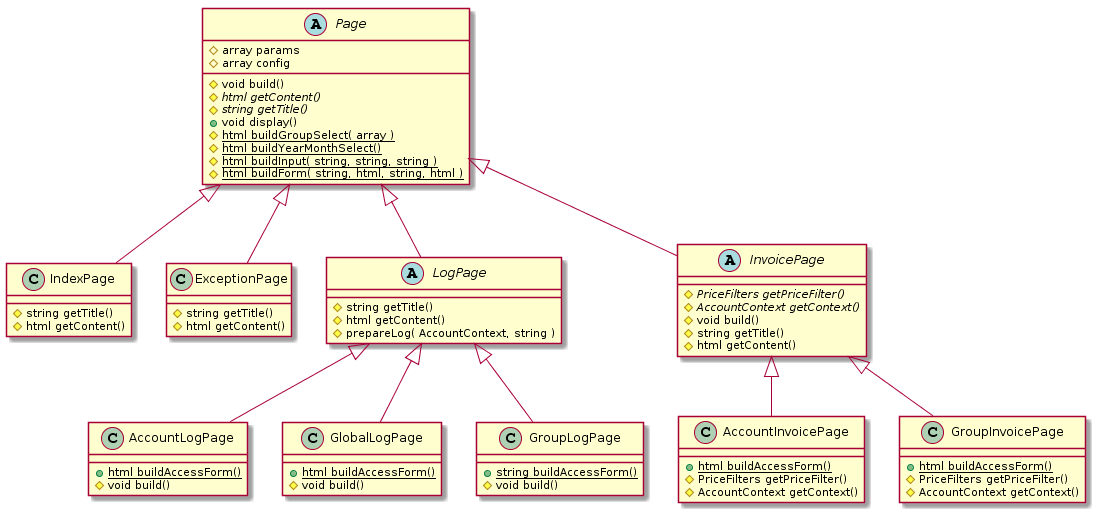
\includegraphics[angle=90, height=18cm]{uml/pages.png}
\end{center}


\end{document}
